\documentclass[a4paper,11pt,spanish,sans]{exam}
\usepackage[spanish]{babel}
%\usepackage[utf8]{inputenc}
\usepackage{multicol}
%\usepackage[latin1]{inputenc}
\usepackage{fontspec}%la posta para las tildes con lualatex
\usepackage[margin=0.5in]{geometry}
\usepackage{amsmath,amssymb}
\usepackage{multicol}
\usepackage{natbib}
\usepackage{graphicx}
\usepackage{hyperref}
\usepackage{epstopdf}
\usepackage{capt-of}
\usepackage[usenames]{color}
%los de aca abajo capaz no los uso
\newcommand{\class}{Matemática: Guía de  Funciones Racionales}
\newcommand{\term}{2° Trimestre 2015}
\newcommand{\examnum}{}
\newcommand{\examprof}{Alexis Gomel}
\newcommand{\examdate}{15/7/2015}
\newcommand{\timelimit}{60 Minutes}%no lo uso
\newcommand{\webpdf}{https://drive.google.com/file/d/0B2MOYme4kZd-Q0VHSTJRb0hINTA/view?usp=sharing}%no lo uso
\newcommand{\Ts}{\rule{0pt}{2.6ex}}       % Top strut
\newcommand{\Bs}{\rule[-1.2ex]{0pt}{0pt}} % Bottom strut

%el header de las hojas.
\pagestyle{head}
\firstpageheader{}{}{}
\runningheader{\class}{\examnum\ - Pagina \thepage\ de \numpages}{\examdate}
\runningheadrule


\begin{document}


\noindent
\begin{tabular*}{\textwidth}{l @{\extracolsep{\fill}} r @{\extracolsep{6pt}} l}
\textbf{\class} & \textbf{Profesor: \examprof}\\

\textbf{PDF: \href{\webpdf}{\textcolor{blue}{http://tinyurl.com/racionales}}} %& Teaching Assistant & \makebox[2in]{\hrulefill}
\end{tabular*}\\
\rule[2ex]{\textwidth}{2pt}

%%%%%%%%%%%%%%%%%%%%%%%%%%%%%%%%%%%%%%%%%%%
%Temas: Racional, Proporcionalidad inversa. Homografica, analisis y construccion. Ecuaciones e inecuaciones. Funcion Irracional. Ecs irracionales. (entran rufinni?, div de polinomios? etc...¿¿¿¿????, meto algo de limites?????; entra el modulo??)
%raices, ordenada al origen, dominio, imagen, crecimiento, decrecimiento, positividad, negatividad. Paridad?
%Hablar de asintotas, 'baches'.

%puedo pedirles un TP con graficos, pidiendo negatividad, positividad, etc... hechos con winplot, mathematica, octave, o lo que sea... Geogebra


\begin{center}
\section*{Guia de Funciónes Racionales}
\end{center}

Definición de una función racional: \[f(x)=\frac{P(x)}{Q(x)}\]
\begin{flushright}
Donde $P(x)$ y $Q(x)$ $(Q(x)\neq 0)$ son polinomios.
\end{flushright}
%Repasar Factoreo.

$Dom(f(x))=\lbrace x \in \mathbb{R} \backslash \:  \: Q(x)\neq 0 \rbrace$ o 
$Dom(f(x))= \mathbb{R} - \lbrace x  \backslash \: \: Q(x)=0\rbrace  $.

Esto se lee: $x$ perteneciente a los números  Reales ($\mathbb{R}$) tal que $Q(x)$ es distinto de $0$; o los reales menos los $x$ tales que $Q(x)$ es igual a $0$.\\ 

Lo cual es esperable, ya que el dominio de los polinomios son todos los reales, tanto para $P(x)$ como para $Q(x)$. Pero tengo que tener cuidado de no dividir por $0$.\\

Ejemplos:\\
 
\begin{minipage}{0.45\textwidth}
$f(x)=\frac{x^2+1}{x-1} \Rightarrow P(x)=x^2+1 \: ; \: Q(x)=x-1$\\
$Dom(f(x))=\mathbb{R} - \lbrace 1\rbrace$

\includegraphics[width= \linewidth]{ejemplo3guia.png}\\

$f(x)=\frac{x^3}{x^4-16} \Rightarrow P(x)=x^3 \: ; \: Q(x)=x^4-16$\\
$Dom(f(x))=\mathbb{R} - \lbrace -2; 2\rbrace$

\includegraphics[width= \linewidth]{ejemplorac5.png}

%$f(x)=\frac{x+5}{x^2-4} \Rightarrow P(x)=x+5 \: \: Q(x)=x^2-4$\\
%$Dom(f(x))=\mathbb{R} - \lbrace -2 ; 2 \rbrace$

%\includegraphics[width= \linewidth]{problema2guia.png}\\

%$f(x)=\frac{x^3+2}{x^4+1} \Rightarrow P(x)=x^3+2 \: \: Q(x)=x^4+1$\\
%$Dom(f(x))=\mathbb{R} $
\end{minipage}
\begin{minipage}{0.45\textwidth}
$f(x)=\frac{1}{x-1} \Rightarrow P(x)=1 \: ; \: Q(x)=x-1 $\\
$Dom(f(x))=\mathbb{R} - \lbrace 1\rbrace$

\includegraphics[width= \linewidth]{racejemplo1.png}\\

$f(x)=2x+3 \Rightarrow P(x)=2x+3 \: ; \: Q(x)=1$\\
$Dom(f(x))=\mathbb{R}$

\includegraphics[width= \linewidth]{ejemplo2.png}
\end{minipage}\\

Las funciones Racionales tiene \textbf{asintota vertical (A.V.)} para cualquier valor $\alpha$ que anule al denominador, pero no al numerador.

Por lo tanto $\alpha$ es \textbf{asintota vertical} $\Leftrightarrow$  $\:\: Q(\alpha)=0 \wedge P(x)\neq 0 $

Mientras que tiene una \textbf{asintota horizontal (A.H.)} , si el grado del numerador ($P(x)$) es menor o igual al grado del denominador($Q(x)$).
La asintota horizontal es $y=0$ cuando el grado de $P(x)$ es menor a $Q(x)$.

En el caso de que $P$ y $Q$ sean del mismo grado. 
Sean $P(x)=a_0+a_1.x+a_2.x^2+......+a_{n-1}.x^{n-1}+a_n.x^n$ y $Q(x)=b_0+b_1.x+b_2.x^2+......+b_{n-1}.x^{n-1}+b_n.x^n$ dos polinomios de grado $n$, la asintota horizontal es $y=\frac{a_n}{b_n}$. \\


Ejemplo de la vida real: El Potencial de \href{https://es.wikipedia.org/wiki/Potencial_de_Lennard-Jones}{\textcolor{blue}{Lennard-Jones}}  $V_{LJ}(r)=[\frac{A}{r^{12}}-\frac{B}{r^6}]$  modela la energía (y por lo tanto la fuerza) que existe en la unión entre dos atomos o dos moleculas, donde $A$ y $B$ son números que se obtienen realizando experimentos.

%\begin{figure}[!h]
%\centering
%\includegraphics[width=0.7\textwidth]{compararlogs.jpg}
%\caption{$log(x)$ en verde, $log_2(x)$ en rojo  y $ln(x)$ en azul.}
%\label{fig:coplogs}
%\end{figure}

\label{inversa}
\emph{Caso particular:} \textbf{Función de proporcionalidad inversa}
\[f(x)=\frac{k}{x}\]
\begin{flushright}
A esta curva se la llama \textbf{Hiperbola}.
\end{flushright}
%Repasar Factoreo.

$Dom(f(x))=\lbrace x \in \mathbb{R} \backslash \:  \: x\neq 0 \rbrace$ o 
$Dom(f(x))= \mathbb{R} - \lbrace 0\rbrace  $.

Esto se lee: $x$ perteneciente a los números  Reales ($\mathbb{R}$), tal que $x$ es distinto de $0$.
Lo cual es esperable, ya que no existe dividir por 0.\\ 

El producto de $y.x$ para cada punto de la curva es constante, ya que $y=\frac{k}{x} \Leftrightarrow y.x=k $. A $k$ se la llama constate de proporcionalidad.



Ejemplo: 
Para envasar 600 litros de jugo, la cantidad de botellas que se necesitan ($y$) es función de la capacidad de botellas a utilizar ($x$). Como la cantidad de botellas que necesito es inversamente proporcional a la capacidad que tiene cada una, esta es una \emph{función de proporcionalidad inversa}. 

(cantidad de botellas)$\times$(capacidad de las botellas)$=600$ litros $\Rightarrow y.x=600$ $\Leftrightarrow y=\frac{600}{x}$

Mientras mas capacidad tengan las botellas, menos botellas necesito para tener $600$ Litros.

\begin{minipage}{0.3\linewidth}

\centering
$y=\frac{600}{x} $\\
$Dom(f(x))=\mathbb{R} - \lbrace 0 \rbrace$\\


\end{minipage}
\begin{minipage}{0.7\linewidth}

\centering
\includegraphics[width= 0.8\linewidth]{inversaej.png}\\

\end{minipage}


\label{homografica}
\emph{Caso Particular:} Si $P(x)$ y $Q(x)$ son ambas \textbf{Polinomios de grado 1} entonces se la llama \textbf{Función Homografica}.

\[f(x) = \frac{a x + b}{c x + d}\]
\begin{flushright}
$Dom(f(x))=\mathbb{R} - \lbrace -\frac{d}{c}\rbrace$
\end{flushright}

\begin{figure}[ht!]
\centering
\includegraphics[width=0.75\textwidth]{homograficaej.png}
\caption{Ejemplo de una función homografica $f(x)=\frac{43x-70}{10x+70}$. En \href{http://tube.geogebra.org/m/1446635}{\textcolor{blue}{Geogebra}} pueden ver un gráfico interactivo de funciones homograficas}
\label{fig:homografica}
\end{figure}

En este caso particular, hay una única \textit{asintota vertical}, que se encuentra en $x=-\frac{d}{c}$.
 
Mientras que la \textit{asintota horizontal} se encuentra en $y=\frac{a}{c}$.\\

Observar que la función de proporcionalidad inversa es un caso particular de las homograficas, ya que con $a=d=0$ $\longrightarrow$ $f(x) = \frac{b}{c x}=\frac{b/c}{x}$.\\



\section*{Ejercicios}

TP: Los que necesiten nota, pueden entregar esta guia de ejercicios resuelta como trabajo practico. Para aprobar el trabajo practico hace falta resolver(justificados) almenos el 70 porciento de cada seccion. 

Los ejercicios con $\bigstar $ son obligatorios, menos el que tiene $\bigstar \bigstar$.


Si se traban con algún ejercicio, pasen al siguiente, y vuelvan al ejercicio difícil mas tarde.
%cosas que voy a buscar: Raices, ordenadas al origen, asintotas. Dom, Im.
%Hacer algún multiple choice.
\section{Encontrar la función:}
\begin{enumerate}
\item Sea un rectángulo de área $10m^2$  y lados $a$ y $b$. Encontrar como varia la longitud del lado $a$ al variar $b$ , y \href{https://tube.geogebra.org/m/1465885}{\textcolor{blue}{graficar}} $a(b)$ explicitando el dominio, la imagen y las asintotas de la función.
\item Si 3 pintores tardan 2 días 15 días en pintar un edificio. Cuanto tardan 4 pintores? 
Encontra una función ($t(p)$) que describa cuanto tarda ($t$) una cierta cantidad de pintores($p$) en pintar el edificio. Graficar.
\item Si un auto  tarda $2hs$ en recorrer $200km$, a que velocidad media tiene que ir para recorrer esos $200km$ en $30min$. Encontrar una función ($t(v)$) que describa el tiempo que tarda el auto en recorrer $200km$ en función de la velocidad media ($v$). Graficar.


\item $\bigstar$ Pensa en un problema en el que tengas que usar una proporcionalidad inversa. Resolvelo y grafica.

\end{enumerate}

%f(x)=\frac{•}{•}

\section{Graficos:}
Graficar (aproximadamente) las siguientes funciones, especificando las asintotas verticales y horizontales; la ordenada al origen y las raíces:


\begin{multicols}{2}

Inversas:
\begin{enumerate}%cambiar funcion %ojo con cuales son asintotas oblicuas
\item $y=\frac{3}{5x-5}$
\item $y=\frac{-2}{2x+2}$
\item $f(x)=\frac{2}{x-1}$
\item $f(x)=\frac{1}{x^2}$

Homograficas:
\item $f(x)=\frac{3x}{x+2}$ $\bigstar$
\item $f(x)=\frac{4x+5}{3x-6}$
\item $f(x)=\frac{x-1}{x+2}$

\columnbreak

Racionales:
\item $f(x)=\frac{x^2(1-x)}{x^2-1}$
\item $f(x)=\frac{3x+1}{x^3+8}$%libro
\item $f(x)=\frac{x^2-4}{2x^2-1}$%libro
\item $f(x)=\frac{x^2+1}{x^2-1}$
\item $f(x)=\frac{x^2-1}{x+2}$
\item $f(x)=\frac{6x^2}{9-x^2}$
\item $\bigstar$ Pensa en una función que tenga almenos dos asintotas verticales pero ninguna asintota horizontal.

\end{enumerate}
\end{multicols}

\section{Completar:}
%aca va una tabla.

%\begin{table*}[ht!]
\begin{center}
%\caption{Completar}
\label{completar}
\begin{tabular}{|l|c|c|c|c|c|}
\hline
                      & A.V. & A.H. & Raíces & Ordenada al Origen & Dominio \Ts \Bs \\ \hline
$y=\frac{1}{x}$  &   &   &   &   &  \Ts \Bs     \\ \hline
$y=\frac{3}{5x-5}$  &   &   &   &   &  \Ts \Bs     \\ \hline
$y=\frac{-2}{2x+2}$  &   &   &   &   &  \Ts \Bs     \\ \hline
$y=\frac{2x-4}{x-1}$  &   &   &   &   &  \Ts \Bs     \\ \hline
$y=\frac{2}{x^2-16}$  &   &   &   &   &  \Ts \Bs     \\ \hline
$y=\frac{1}{-x^2+x+2}$  &   &   &   &   &  \Ts \Bs     \\ \hline
$y=\frac{2}{4x^2-8x+3}$  &   &   &   &   &  \Ts \Bs     \\ \hline
$y=\frac{3}{x^2-x+2}$  &   &   &   &   &  \Ts \Bs     \\ \hline
$y=\frac{2x^2+3x-4x^3}{5x^2+4}$  &   &   &   &   &  \Ts \Bs     \\ \hline
$y=\frac{4(x+2)(x+3)}{(x-3)(x-1)(x+1)}$   &   &   &   &   &   \Ts \Bs     \\ \hline
$y=-\frac{5(x+1)(x-1)}{(x-3)}$   &   &   &   &   &   \Ts \Bs     \\ \hline
\end{tabular}
%\end{table*}
\end{center}

%elegir otro ejemplo, capaz el del examen, asi lo tiene visto.
%\item Cual de estos gráficos corresponde a $f(x)=\frac{6x-1}{2x+1}$
%
%\begin{figure}[h!]
%\centering
%\includegraphics[width=0.55\textwidth]{encontrarlog3xmas1.jpg}
%\caption{Encontrar $a$,$b$ y $c$,  a partir del gráfico de $y=log_(a)(x-b)$.
%Los asteriscos azules marcan el valor de $y$ para $-1.00001, 2 , 3, 4, 5, 6...$}
%\label{fig:logaritmo}
%\end{figure}
%\end{enumerate}

\section{Cual función corresponde al gráfico.} 
%aca va una tabla y unos graficos

\begin{minipage}{0.45\textwidth}
\centering
%\begin{table}[!h]
%\caption{mc1}
\label{mc1}
\begin{tabular}{|c|c|c|}
\hline
$\frac{x+1}{x^2+4}$  & $\frac{x+1}{x^2-4}$ & $\frac{x+4}{x^+1}$\Ts \Bs   \\ \hline
   &   &      \\ \hline
\end{tabular}\\
%\end{table}
%\begin{figure}[h]
\centering
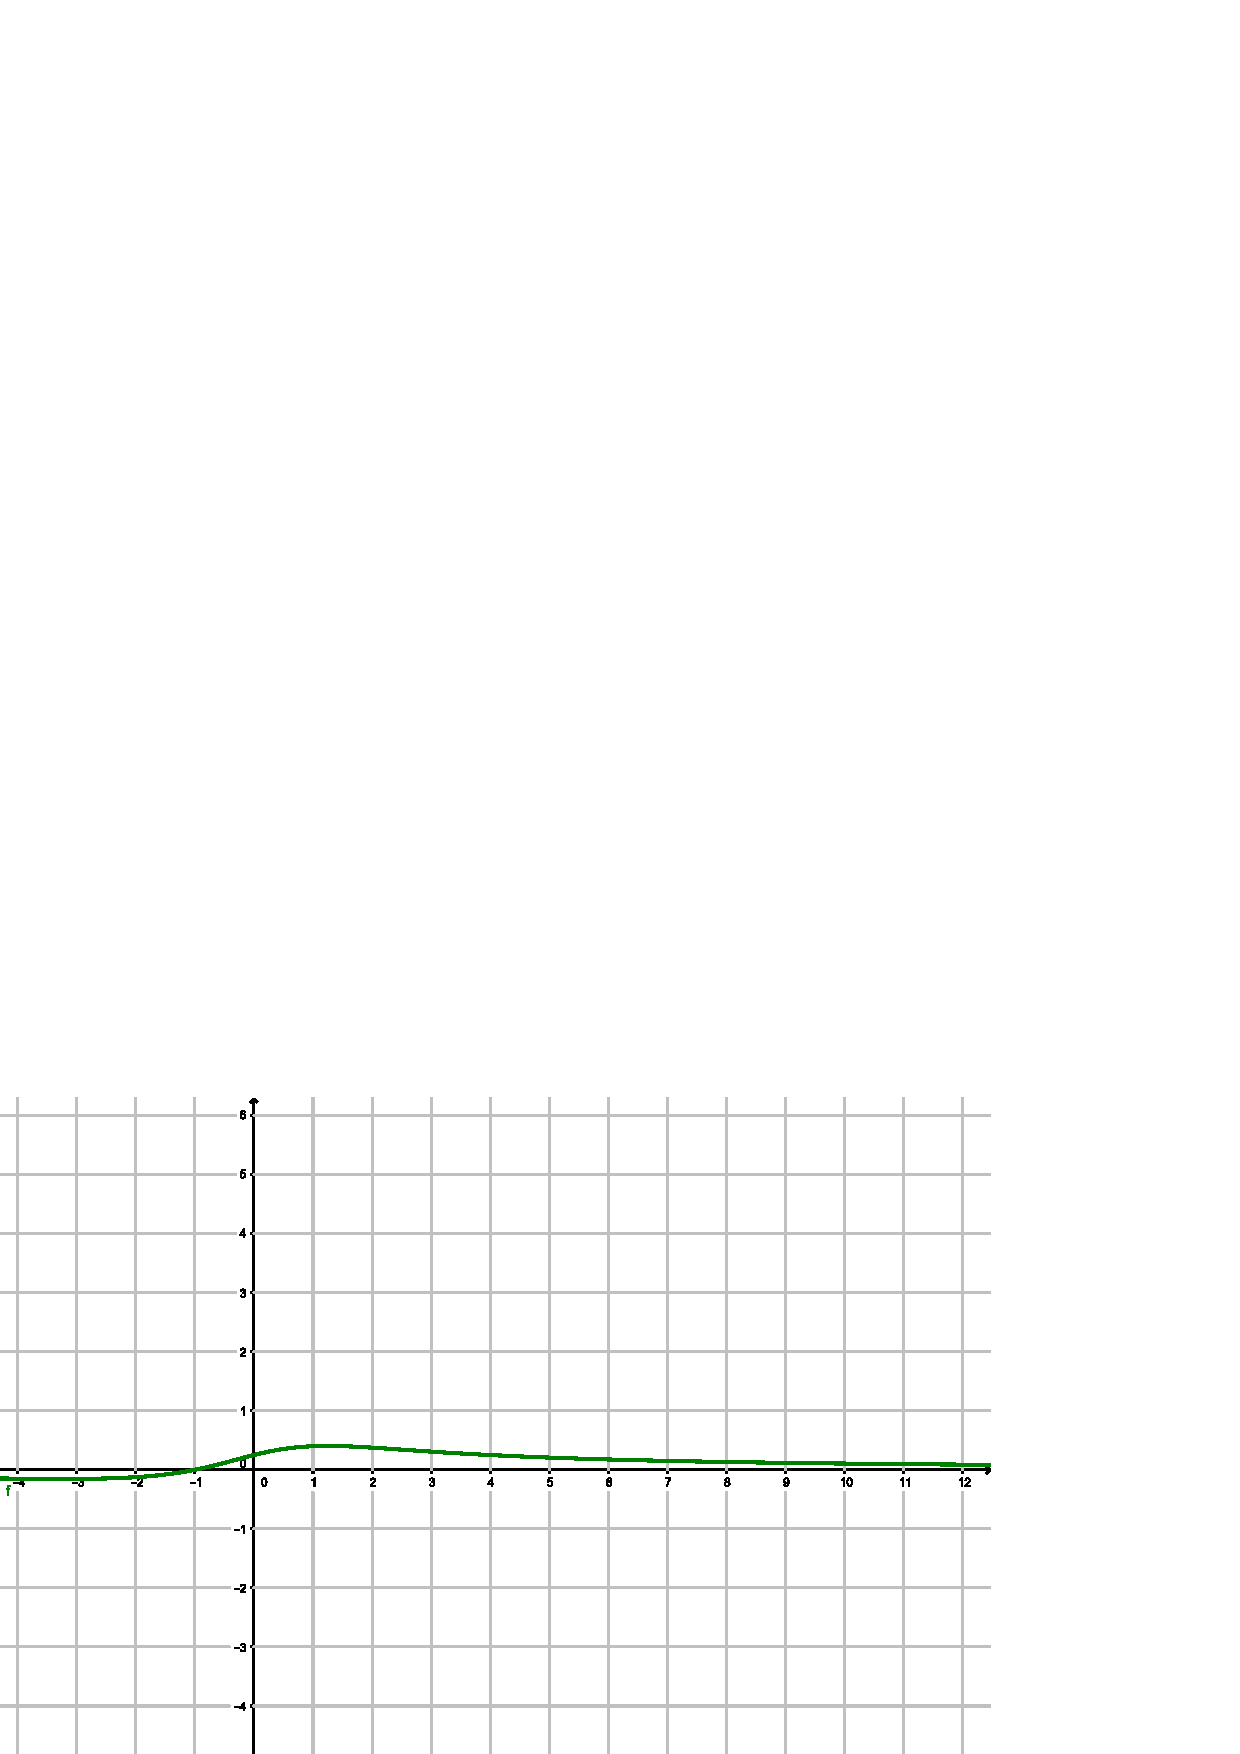
\includegraphics[width= 0.9\linewidth]{primerproblema.png}
%\end{figure}
%graficos
\end{minipage}
\begin{minipage}{.45\textwidth}
\centering
%\begin{table}[!h]
%\caption{mc1}
%\label{mc1}
\begin{tabular}{|c|c|c|}
\hline
$\frac{x^2-9}{2x^2-7}$  & $\frac{x^2+9}{x^2-7}$ & $\frac{2x^2-7}{x^2-9}$ \Ts \Bs  \\ \hline
   &   &      \\ \hline
\end{tabular}\\
%\end{table}
%\begin{figure}[h]
\centering
\includegraphics[width= 0.9\linewidth]{problema2guia.png}
%\end{figure}
\end{minipage}

%grafico
%hacer multicol

\section{Encontrar, si es posible, el valor de x :}

\begin{enumerate}
\begin{multicols}{2}

\item $\frac{5x+4}{2x-1}=1$
\item $\frac{3x-1}{x+1}=10$

\columnbreak

\item $\frac{x^2-x-1}{x^3+x+3}=3$
\item $\frac{1}{x^2+2} + \frac{1}{x^3} =4 $
\item $\frac{1}{x^2+2} + \frac{1}{x} =4 $
\item $\frac{x+2}{x^2-4}=-\frac{1}{2}$



\end{multicols}
\end{enumerate} 

\section{Inecuaciones}

\begin{enumerate}
\begin{multicols}{3}
\item $5x+4 > 2x-1 $
\item $\frac{3}{x} > -2 $
\item $2x^2-8 < x^2-2x+7$
\item $\frac{3x-1}{x+1} < 3$
\item $\dfrac{1}{x} \leq \dfrac{2x+1}{3x}$


\columnbreak

\item $\frac{2}{x^2}\geq 1$
\item $\frac{4}{x} < x-3$
\item $\frac{1}{x} >  2+1-\frac{5}{x}$
\item $\dfrac{x^2+4}{x+2} \leq x$

\columnbreak

\includegraphics[width= 0.7\columnwidth]{algebraic.png}
%\caption{Set joke}
\label{fig:algeb}

\end{multicols}
\end{enumerate} 

\section{Ejercicios Teóricos}.$\bigstar$  $\bigstar$
Teorema: Sean $f(x)$ y $g(x)$ funciones racionales. Entonces $f+g$, $f.g$ y $f(g(x))$ también son funciones racionales. Si $g(x) \neq 0 $, $f/g$ también es una función racional.


\begin{enumerate}

\item Dadas $f(x)=(1+x)/(1-x)$ y $g(x)=1+x^2$, Calcular $f+g$, $2.f$, $f.g$, $f(g(x))$ y mostrar que son funciones racionales.

\end{enumerate}



\rule[2ex]{\textwidth}{2pt}


Observación: Para saber si hiciste bien un ejercicio, reemplaza por tu valor de x.



\section*{Extra y curiosidades}

%El numero $e\simeq$ ..  breve bio de euler-
\begin{itemize}
\item Para que sirven las matemáticas? Charla TED de Eduado Saenz de Cabezon \href{https://www.youtube.com/watch?v=jej8qlzlAGw}{\textcolor{blue}{ $"$Las matemáticas son para siempre$"$}}.

\item El 6 de agosto se cumplió el 70 aniversario del bombardeo nuclear a Hiroshima y el 9 de agosto a Nagasaki. Como forma de conmemoración , y para tomar conciencia, desde  \href{http://nuclearsecrecy.com/nukemap/}{\textcolor{blue}{esta pagina} puede ver una simulación que consecuencias tendría tirar una bomba nuclear en la ciudad que quieran.}

 

\begin{minipage}{0.5\textwidth}

\centering
\includegraphics[width= 0.8\linewidth]{esch.jpg}
%\caption{Cuadro de Escher}
\label{fig:univerise}

\end{minipage}
\begin{minipage}{0.5\textwidth}

\centering
\includegraphics[width= 0.7\linewidth]{mathjokegraph.png}
%\caption{Set joke}
\label{fig:erise}

\end{minipage}

\end{itemize}

%\bibliographystyle{plain}
%\bibliography{references}



\section*{Apéndice}
\subsection*{Casos de Factoreo}

$a^2-b^2=(a+b)(a-b)$

$(a+b)^2=a^2+2ab+b^2$

\subsection*{Formas de la lineal y la cuadrática}

Lineal:

$y=m.x+b$

$y=A(x-r_1)$

Cuadrática:

$y=ax^2+bx+c$

$y=A(x-r_1)(x-r_2)$

$y=C(x-x_v)^2+y_v$




\newpage
%
%\section*{Resultados}
%\begin{enumerate}
%\item
%\begin{enumerate}
%\item -7 ; \item 16 ; \item .. ; \item $3/5$ ; \item 25 ; \item $64/9$ ; \item $c^b $ ;\item $k$ ;\item $\frac{b.d}{c^h} $  ;\item $b=1/c$ ;\item  $2.2,3$ ;\item $2-2,3 = 0,3$ ;\item 2,3/2 ;\item  4,6 ;\item 1$/2,3$ ;\item m/n ;\item  ; 
%\end{enumerate}
%
%\item 
%\begin{enumerate}
%\item
%\item
%\item $log_3(x+1)$
%\end{enumerate}
%
%\item
%\begin{enumerate}
%\item $x=8$
%\item $-2/3$
%\item $x=5$
%\item $x=9$
%\item 
%\item 
%\item $x=2$
%\item $x=2$
%\item $x=1$,$x=$ 
%\end{enumerate}
%
%\item
%
%\item 
%
%


\end{document}